\documentclass[xcolor=table, aspectratio=169]{beamer}
\usepackage{beamerthemesplit}
\usepackage{wrapfig}
\usetheme{SPbGU}
\usepackage{pdfpages}
\usepackage{amsmath}
\usepackage{cmap}
\usepackage[T2A]{fontenc}
\usepackage[utf8]{inputenc}
\usepackage[english]{babel}
\usepackage{indentfirst}
\usepackage{amsmath}
\usepackage{tikz}
\usepackage{multirow}
\usepackage[noend]{algpseudocode}
\usepackage{algorithm}
\usepackage{algorithmicx}
\usepackage{fancyvrb}
\usetikzlibrary{shapes,arrows}
%usepackage{fancyvrb}
%\usepackage{minted}
%\usepackage{verbments}
\usepackage{fontawesome}
\usepackage{xcolor}


\beamertemplatenavigationsymbolsempty

\title[FL guided data analysis group results]{Formal language guided data analysis group results}
\institute[SPbU]{
JetBrains Research, Programming Languages and Tools Lab  \\
St. Petersburg University
}

\author[Semyon Grigorev]{Semyon Grigorev}

\date{18.12.2021}

\begin{document}
{
\begin{frame}[fragile]
  \begin{tabular}{p{2.0cm} p{9.5cm} p{1cm}}
   \begin{center}
      
\includegraphics[height=1.5cm]{pictures/jetbrainsResearch.pdf}
    \end{center}
    &
    \begin{center}
      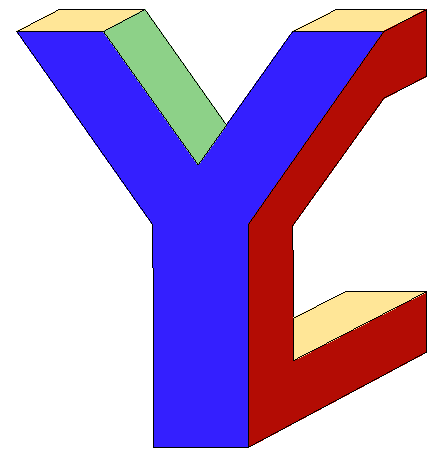
\includegraphics[height=1.5cm]{pictures/YC_logo.pdf}
    \end{center}
    &
    \begin{center}
      
\includegraphics[height=1.5cm]{pictures/SPbGU_Logo.png}
    \end{center}
  \end{tabular}
  \titlepage
\end{frame}
}


\begin{frame}[fragile]

  \frametitle{Research Interests}
\begin{itemize}
      \item Formal language theory, parsing algorithms
      \item Sparse linear algebra and parallel computations
      \item Program optimization methods: supercompilation, distillation, etc (in collaboration with Daniil Berezun)
      \item Application of all above for
      \begin{itemize}
        \item Static code analysis
        \item Graph databases
        \item Biological data analysis
        \item \ldots
      \end{itemize}

\end{itemize}

\end{frame}

\begin{frame}[fragile]

  \frametitle{Team}
\begin{itemize}
      \item PhD students
      \begin{itemize}
        \item Rustam Azimov
        \item Ekaterina Shemetova
      \end{itemize}
      \item Master students
      \begin{itemize}
        \item Alexandra Istomina
        \item Egor Orachev
        \item Ilya Epelbaum
        \item Vladimir Kutuev
        \item \textcolor{gray}{Arseniy Terekhov $\to$ CLion team}
      \end{itemize}
      \item Bachelor students
      \begin{itemize}
        \item Vlada Pogozhelskaya
        \item Vadim Abzalov
        \item Timur Zinnatulin
        \item Dmitriy Panfilyonok
        \item Artem Chernikov
      \end{itemize}
      \item About six 2nd, 3rd, 4th year students: graduate projects, semester practices, etc
\end{itemize}

\end{frame}


\begin{frame}[fragile]
\frametitle{Conferences}
\begin{itemize}

      \item[\faCheck] \textbf{EDBT-2021} (CORE A) 
      \begin{itemize}
        \item Arseniy Terekhov, Vlada Pogozhelskaya, Vadim Abzalov, Timur Zinnatulin, \emph{Semyon Grigorev}. Multiple-Source Context-Free Path Querying in Terms of Linear Algebra
        \item Scopus
      \end{itemize}
        
      \item[\faCheck] \textbf{LDBC TUC 2021}
      \begin{itemize}
         \item \emph{Semyon Grigorev}. Context-Free Path Querying: Obstacles on the Way to Adoption
         \item Invited by Gabor Szarnyas
      \end{itemize}

      \item[\faCheck] \textbf{GrAPL-2021}
      \begin{itemize}
         \item \emph{Egor Orachev}, Maria Karpenko, Artem Khoroshev, Semyon Grigorev. SPbLA: The Library of GPGPU-Powered Sparse Boolean Linear Algebra Operations
         \item Scopus
      \end{itemize}

    \end{itemize}
    \end{frame}


\begin{frame}[fragile]

  \frametitle{Conferences}
      \begin{itemize}

      \item[\faCheck] \textbf{GRADES-NDA 2021}
      \begin{itemize}
        \item \emph{Rustam Azimov}, Ilya Epelbaum, Semyon Grigorev. Context-Free Path Querying with All-Path Semantics by Matrix Multiplication
        \item Scopus
      \end{itemize}

      \item[\faCheck] \textbf{VLDB PhD Workshop 2021}
      \begin{itemize}
         \item \emph{Rustam Azimov}. Context-Free Path Querying In Terms of Linear Algebra
         \item Scopus
      \end{itemize}

      \item[\faHourglassHalf] \textbf{EDBT-2022} (CORE A) 
      \begin{itemize}
        \item Vlada Pogozhelskaya, Anna Vlasova, Semyon Grigorev. GLL-based Context-Free Path Querying for Neo4j
        \item Submitted
      \end{itemize}

\end{itemize}
\end{frame}

\begin{frame}[fragile]

  \frametitle{Collaboration}
\begin{itemize}
      \item Internal
      \begin{itemize}
        \item Daniil Berezun: distillation of linear algebra based algorithms
        \item Anton Podkopaev: Graph Query Language semantics formalization and mechanization in Coq
      \end{itemize}
      \item External
      \begin{itemize}
      \item Alexander Okhotin, RSF grant 
      \begin{itemize}
        \item Semyon Grigorev,Ekaterina Shemetova
      \end{itemize}
      \item LDBC community
      \begin{itemize}
        \item Formal languages constrained path querying algorithms
        \item Competition of FL constrained path querying algorithms 
      \end{itemize}
      \item Neo4j team
      \begin{itemize}
        \item CFPQ for Neo4j
      \end{itemize}
    \end{itemize}

\end{itemize}
\end{frame}

\begin{frame}[fragile]

  \frametitle{Teaching}
\begin{itemize}
      \item Formal language theory (lectures, seminars): SPbU
        \begin{itemize}
          \item [\faGears] Lecture notes (in collaboration with Ekaterina Verbitskaia): \url{https://github.com/JetBrains-Research/FormalLanguageConstrainedReachability-LectureNotes} 
          \item [\faGears] Exercises and supplementary materials (in collaboration with Egor Orachev and Vadim Abzalov): \url{https://github.com/JetBrains-Research/formal-lang-course}
        \end{itemize}
      \item Graph theory: SPbU
      \item Formal language theory seminar
      \item Graduation projects, practices, semester projects for students from CSC, HSE, SPbU, ITMO, etc
\end{itemize}
\end{frame}

\begin{frame}[fragile]

  \frametitle{Grants}
\begin{itemize}
      \item[\faTimes] RSF 
      \begin{itemize}
        \item ``Sparse linear algebra: from specialized hardware to applied solutions''
        \item Semyon Grigorev, Daniil Berezun, Anton Podkopaev, Timofey Briksin, Rustam Azimov, Egor Orachev, Alexey Turin, Arceniy Terekhov
      \end{itemize}
\end{itemize}
\end{frame}

\begin{frame}[fragile]

\frametitle{Work in progerss: publications}
\begin{itemize}
      \item[\faHourglassHalf] Ekaterina Shemetova, Alexander Okhotin, Semyon Grigirev. Rational index of bounded-oscillation languages. Arxiv: \url{https://arxiv.org/abs/2012.03567}
      
      \item[\faHourglassHalf] Ekaterina Shemetova, Rustam Azimov, Egor Orachev, Ilya Epelbaum, Semyon Grigorev. One Algorithm to Evaluate Them All: Unified Linear Algebra Based Approach to Evaluate Both Regular and Context-Free Path Queries. Arxiv: \url{https://arxiv.org/abs/2103.14688}
      \item[\faHourglassHalf] Polina Lunina, Vadim Abzalov, Semyon Grigorev. Genegram: RNA Secondary Structure       Prediction Using Formal Grammars and Residual Neural Networks
      \pause
      \item[\faGears] Egor Orachev and Gleb Mar'in. On multi-GPU sparse linear algebra
      \item[\faGears] Dmitriy Panfilyonok and Artem Chernikov. On On functional languages based design of generic sparse linear algebra routines 
      \item[\faGears] Alexey Turin, Ekaterina Vinnik, Daniil Berezun. On distillation of sparse lianear algebra routines
      \item[\faGears] $\ldots$
\end{itemize}
\end{frame}

\begin{frame}[fragile]

  \frametitle{Work in progress: main directions}
\begin{itemize}
      \item Linear algebra based algorithms for formal language constrained path querying development and evaluation
      \item Time complexity of context-free path querying
      \item Formal semantics of graph query languages (in collaboration with Anton Podkopaev) 
      \item Applications of formal language constrained path querying (graph databases, staic code analysis, bioinormatics)
      \item Fast sparse linear algebra
      \begin{itemize}
        \item Parallel and GPGPU programming, and techniques to do it fast and safe
        \item Optimization techniques and specialized hardware: distillation, lambda-precessors (in collaboration with Daniil Berezun)
      \end{itemize}
\end{itemize}
\end{frame}

\end{document}
